\documentclass[aps,superscriptaddress,tightenlines,nofootinbib,floatfix,longbibliography,notitlepage]{revtex4-1}
\usepackage[left=18mm,right=19mm,top=23mm,bottom=16mm]{geometry}
\usepackage{amsmath,amssymb}
\usepackage{bm}
\usepackage{comment}
\usepackage{graphicx}
\usepackage[dvipsnames]{xcolor}
\usepackage{slashed}
\usepackage[
    colorlinks=true,
    allcolors=blue
]{hyperref}



%%%
%%%     Incorporate Repository Information
%%%

\providecommand{\repositoryInformationSetup}{} % Fallback definition if compiled with `make FINAL=1`.
\repositoryInformationSetup

%%%
%%%     Include latex-base macros
%%%

\usepackage{xspace}
\usepackage{bbm}

%%%%
%%%%    Project Specifics
%%%%

\newcommand{\repoURL}{https://github.com/evanberkowitz/latex-base}

%%%%
%%%%    Referring to Parts of the Document
%%%%

\newcommand{\secref}[1]{Sec.~\ref{sec:#1}}
\newcommand{\Secref}[1]{Section~\ref{sec:#1}}
\newcommand{\appref}[1]{App.~\ref{sec:#1}}
\newcommand{\Appref}[1]{Appendix~\ref{sec:#1}}
\newcommand{\tabref}[1]{Tab.~\ref{tab:#1}\xspace}
\newcommand{\Tabref}[1]{Table~\ref{tab:#1}\xspace}
\newcommand{\figref}[1]{Fig.~\ref{fig:#1}\xspace}
\newcommand{\Figref}[1]{Figure~\ref{fig:#1}\xspace}
\renewcommand{\eqref}[1]{(\ref{eq:#1})\xspace}
\newcommand{\Eqref}[1]{Equation~\ref{eq:#1}\xspace}
\def\Ref#1{Ref.~\cite{#1}} % Use \def because some LaTeX installations define \Ref, others do not.
\newcommand{\Reference}[1]{Reference~\cite{#1}}
\newcommand{\Refs}[1]{Refs.~\cite{#1}}
\newcommand{\References}[1]{References~\cite{#1}}

%%%%
%%%%    Referring to Parts of the GitHub Repository
%%%%

\newcommand{\issue}[1]{\href{\repoURL/issues/#1}{Issue #1}}
\newcommand{\pullrequest}[1]{\href{\repoURL/pulls/#1}{Pull Request #1}}

%%%%
%%%%    Referring to Other Documents
%%%%

\renewcommand{\doi}[1]{\href{http://doi.org/#1}{[#1]}}
\newcommand{\arxiv}[1]{\href{http://www.arxiv.org/abs/#1}{arXiv:#1}}

%%%%
%%%%    Mathematical Symbols
%%%%

\newcommand{\goesto}{\ensuremath{\rightarrow}}
\newcommand{\infinity}{\infty}
\newcommand{\Integers}{\mathbb{Z}\xspace}
\newcommand{\integers}{\Integers}
\newcommand{\one}{\ensuremath{\mathbbm{1}}}
\newcommand{\order}[1]{\ensuremath{\mathcal{O}\left(#1\right)}\xspace}
\newcommand{\Rationals}{\mathbb{Q}\xspace}
\newcommand{\Reals}{\mathbb{R}\xspace}
\newcommand{\union}{\ensuremath{\cup}}
\DeclareMathOperator{\erf}{erf}
\renewcommand{\mod}[1]{\ensuremath{\ \left(\text{mod }#1\right)}}

%%%%
%%%%    Hyperbolic Trig
%%%%

% Most are already available if you \usepackage{amsmath}.
% However, those below are missing

\DeclareMathOperator{\sech}{sech}
\DeclareMathOperator{\csch}{csch}
\DeclareMathOperator{\arccosh}{arccosh}
\DeclareMathOperator{\arcsinh}{arcsinh}
\DeclareMathOperator{\arctanh}{arctanh}
\DeclareMathOperator{\arcsech}{arcsech}
\DeclareMathOperator{\arccsch}{arccsch}
\DeclareMathOperator{\arccoth}{arccoth}

% Additionally, there are some missing trig functions:

\DeclareMathOperator{\arcsec}{arcsec}
\DeclareMathOperator{\arccot}{arccot}
\DeclareMathOperator{\arccsc}{arccsc}

%%%%
%%%%    Fractions
%%%%

\newcommand{\oneover}[1]{\ensuremath{\frac{1}{#1}}}                             %   1/[argument]
\newcommand{\inverse}{\ensuremath{^{-1}}}                                       %   argument^-1
\newcommand{\half}{\ensuremath{\frac{1}{2}} }                                   %   1/2
\newcommand{\quarter}{\ensuremath{\frac{1}{4}} }                                %   1/4


%%%%
%%%%    Mathematical Delimiters
%%%%
\newcommand{\abs}[1]{\ensuremath{\left| #1 \right|}\xspace}
\newcommand{\magnitude}{\abs}
\newcommand{\average}[1]{\ensuremath{\left\langle #1 \right\rangle}\xspace}

% Quantum mechanics bra-ket notation:
\newcommand{\ket}[1]{\ensuremath{\left|\;#1\;\right\rangle}}
\newcommand{\bra}[1]{\ensuremath{\left\langle\;#1\;\right|}}
\newcommand{\bracket}[2]{\ensuremath{\left\langle\;#1\;\middle|\;#2\;\right\rangle}}
\let\braket\bracket


%%%%
%%%%    Matrices
%%%%

\newcommand{\identity}{\ensuremath{\mathds{1}}}
\newcommand{\diag}[1]{\ensuremath{\text{diag}\left(#1\right)}}
\newcommand{\tr}[1]{\ensuremath{\text{tr}\left[#1\right]}}
\newcommand{\transpose}{\ensuremath{{}^{\top}}}
\newcommand{\adjoint}{\ensuremath{{}^{\dagger}}}

%%%%
%%%%    Physical Quantities and Constants
%%%%




%%%%
%%%%    Software
%%%%

\newcommand{\bash}{\texttt{bash}\xspace}
\newcommand{\git}{\texttt{git}\xspace}
\newcommand{\make}{\texttt{make}\xspace}
\newcommand{\mpi}{\texttt{MPI}\xspace}
\newcommand{\python}{\texttt{python}\xspace}

% Put an xspace after \LaTeX:
\let\builtinLaTeX\LaTeX
\def\LaTeX{\builtinLaTeX\xspace}
 % input rather than include so we don't create macros.aux

%%%%
%%%%    Document preparation
%%%%


\begin{document}

\title{Example \LaTeX + \texttt{git} }

\author{Evan Berkowitz}

\date{\today}

\begin{abstract}
Here's a bare-bones example where I set up a \git repo with all the \LaTeX-related things that I like.
\end{abstract}

\maketitle

\section{Introduction}\label{sec:intro}

\LaTeX is a system for producing beautiful documents.
It takes as input a set of plain text files, and produces a variety of output types; the most useful to me is PDF.

\git is a decentralized version control system.
It's fantastic.
There is a version control package, \texttt{vc}\cite{vc} which provides some of the same functionality provided here; you may be better off with that, depending on your use case.

This repo\cite{latex-base} is an example that is supposed to make it easy to make \git-controlled \LaTeX documents.
In particular, I have used a GitHub action that checks that pushed commits and pull requests successfully produce a PDF.
That helps keep everybody\ldots\ on the same page.

\section{Version Control Information}\label{sec:vc}

There is a small shell script that reports the status of the repo when the PDF is being compiled.
The script \texttt{repo/git.sh} produces some \LaTeX which, in the current example, like
\begin{verbatim}
\newcommand{\repositoryInformationSetup}{
    \usepackage[dvipsnames]{xcolor}
    \usepackage[ angle=90, color=black, opacity=1, scale=2, ]{background}
    \SetBgPosition{current page.west}
    \SetBgVshift{-4.5mm}
    \backgroundsetup{contents={{\color{Red}3 files in \texttt{-{}-} different from commit \
        \texttt{HEAD} from 2019-01-22 10:35:10 +0100}}}
}
\end{verbatim}

By adding additional scripts in the \texttt{repo} directory and changing the \texttt{REPO} makefile variable from \git to a version control system of your choice, you can extend the ability of this skeleton to provide information about the state of the repository.
The script must simply return \texttt{{\textbackslash}repositoryInformationSetup}.
How the \texttt{{\textbackslash}repositoryInformationSetup} is smuggled into the \TeX\ itself is discussed in \Secref{make} on \texttt{make}.

\texttt{repo/git.sh} takes two ordered, optional arguments.  \texttt{OLD} and \texttt{NEW}, which allows you to specify which commits you wish to compare.  They default to \texttt{HEAD} and \texttt{-{}-}, respectively, so that the default behavior compares the current state of the repository with the latest commit.  This is useful with the \texttt{DIFF} flag for \texttt{make}, discussed in \Secref{make}.

To get the \git status on the left margin of every page I simply invoke \texttt{make}.
One may invoke \texttt{\make FINAL=1} or use, for example, \texttt{pdflatex master.tex}, to produce a PDF without the \git information in the margin.

\section{Makefile}\label{sec:make}

The provided \texttt{Makefile} uses \texttt{pdflatex} and \texttt{bibtex} to compile \texttt{master.pdf}, the base of which is set in the \texttt{MASTER} variable.
You can change the executables in the \texttt{TEX} and \texttt{BIB} variables.  It has been carefully constructed so that if the user (or, say, their collaborators) do not compile using the \texttt{Makefile}, nothing bad happens or goes wrong.

\subsection{Targets}

The default target is \texttt{\$(MASTER).pdf}, drawn from \texttt{\$(MASTER).tex}.
You can add other root-level documents and simply do \texttt{make other-document.pdf} without adding new rules to the \texttt{Makefile}.
The PDF targets depend on the files in the \texttt{section} directory, \texttt{macros.tex}, all \texttt{.bib} files in the repository, and the corresponding root-level \texttt{tex} document.

The \texttt{tidy} target gets rid of temporary files generated by \LaTeX, while the \texttt{clean} target gets rid of additional files and the generated PDF.  Both understand the \texttt{TARGET} flag.

The \texttt{watch} target monitors the repository for file changes and continuously rebuilds \texttt{\$(TARGET).pdf}.  It relies on \texttt{when-changed}\cite{when-changed}.
It can get stuck in an infinite loop if the PDF does not compile correctly.
But if you tend to write decent \LaTeX the first time around, it'll be pretty reliable.


\subsection{User Flags}

The \texttt{TARGET} variable defaults to \texttt{\$(MASTER)} but can be overridden.  It is useful for the \texttt{tidy}, \texttt{clean}, and \texttt{watch} targets.
It should take the value of the prefix of the PDF file you wish to generate; if you want to continuously generate \texttt{foo.pdf} and \texttt{foo.tex} is at the root level of the repo, you can simply do \texttt{make watch TARGET=foo}.
The \texttt{tidy} and \texttt{clean} targets operate similarly.

The \texttt{FINAL} variable controls whether the result of \texttt{./repo/\$(REPO).sh} is used as part of the preamble to the \texttt{tex} file.  The result is used by default, set \texttt{FINAL=1} to remove it.

The \texttt{DIFF} variable decides whether the resulting PDF indicates differences between the \texttt{OLD} and \texttt{NEW} repository states, using \texttt{git latexdiff}\cite{git-latexdiff}.  \texttt{OLD} defaults to the SHA of the latest commit and \texttt{NEW} to \texttt{-{}-}, indicating the current state of the repo (including unstaged changes, but NOT including untracked files).  In this repo, for example, you can
\begin{verbatim}
	make DIFF=1 OLD=df58f60 NEW=93d2abc
\end{verbatim}
If \texttt{OLD} is later than \texttt{NEW}, I don't know what happens in general.
If you use a different version control system, you should change the defaults for \texttt{OLD} and \texttt{NEW} (and, presumably change the diff generator to something other than \texttt{git latexdiff}).

\subsection{Other \texttt{Makefile} Variables}

There are variables in the \texttt{Makefile} that presumably don't need to change once they're set.
The \texttt{REPO}, \texttt{OLD}, \texttt{NEW}, \texttt{ROOT}, and \texttt{MASTER} variables are examples.

The \texttt{SHORTCIRCUIT} variable should not be used by the user.
The difficulty was that once the user sets the \texttt{DIFF} flag, \texttt{git latexdiff} uses the \texttt{Makefile} to build the diff, and the \texttt{DIFF} flag is passed along.  So, \texttt{git latexdiff} would be invoked in an infinite loop.
Defining \texttt{SHORTCIRCUIT} breaks that loop.

\section{GitHub Action}

A GitHub action is something that automatically happens when the status of a git repository changes on GitHub.
GitHub actions can be used to compile executables, run tests, deploy services, and do other automatic things.
This repository uses an action to compile a PDF!

We use an action called \texttt{latex-action}~\cite{latex-action} which uses a maximal TeXLive environment (meaning that most packages will already exist in the TeX installation).
If you need a non-standard LaTeX package, you can \texttt{apt-get} it---see the action's \href{https://github.com/dante-ev/latex-action/blob/master/README.md}{\texttt{README.md}} for details.

This action runs when code is \texttt{push}ed, or a branch is \texttt{pull\_request}ed.  You can adjust the events that trigger this action by changing the \texttt{on} setting of \href{https://github.com/evanberkowitz/latex-base/blob/master/.github/workflows/main.yml}{.github/workflows/main.yml}.

To check that the PDF's source code is correct, this action attempts to compile it.  You can choose the compilation target by adjusting \texttt{jobs:env:target} from \texttt{master} to your preferred target, again in \href{https://github.com/evanberkowitz/latex-base/blob/master/.github/workflows/main.yml}{.github/workflows/main.yml}.

This action produces an \emph{artifact}---something that survives after the automatic action is finished.
It creates a PDF that you can look at!

To see this PDF, you need to look at the checks of the commit (or pull request).
To find the details of the checks, find the symbol next to the commit---it might be a red X (indicating a failure), a yellow dot (indicating that the action is in progress), or a green check (indicating the action succeeded).
Click that symbol and then click `details', as suggested in the screenshot below.
\begin{center}
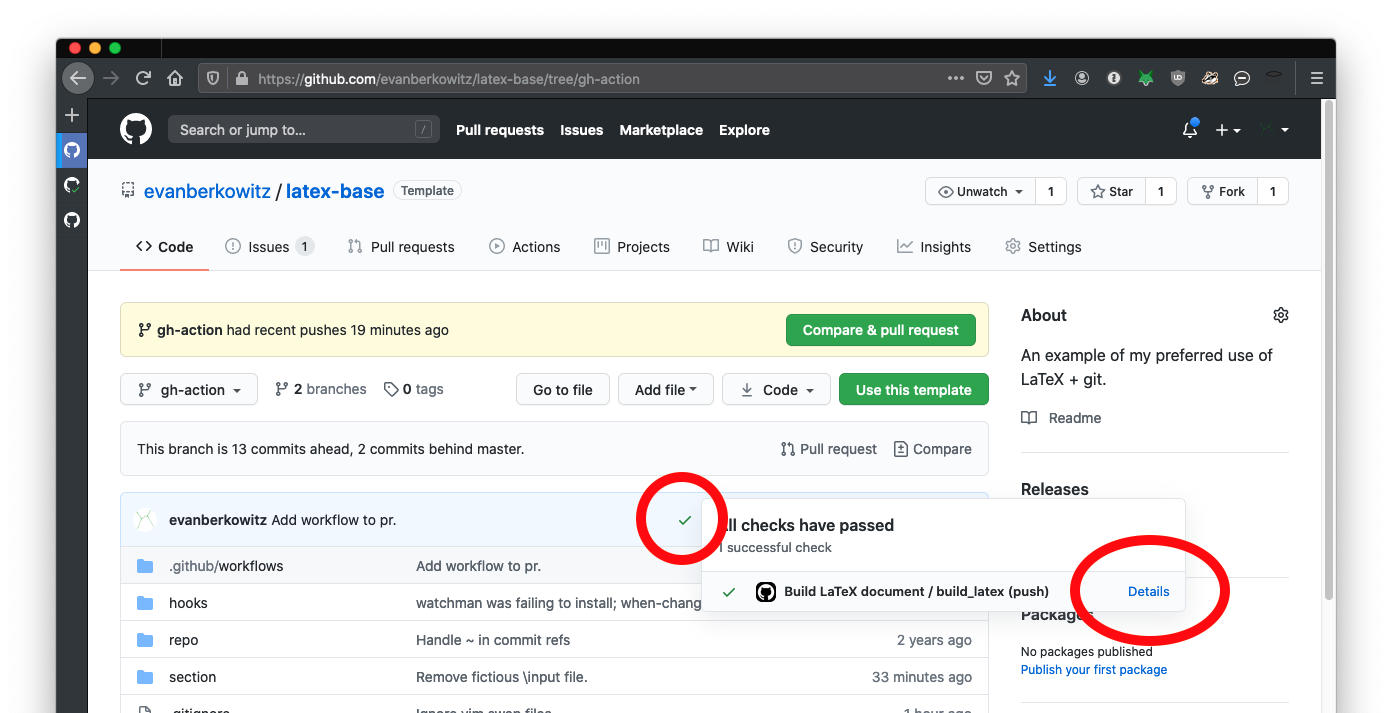
\includegraphics[width=0.75\textwidth]{figure/github-action-find-details}
\end{center}
To see the PDF, one must download the artifact, as shown in the screenshot below.
Artifacts are named after the target, and are suffixed with the SHA of the commit.
Artifacts are always ZIP files.  When you unzip it you will see a PDF, which reflects the state of the code after that commit.
\begin{center}
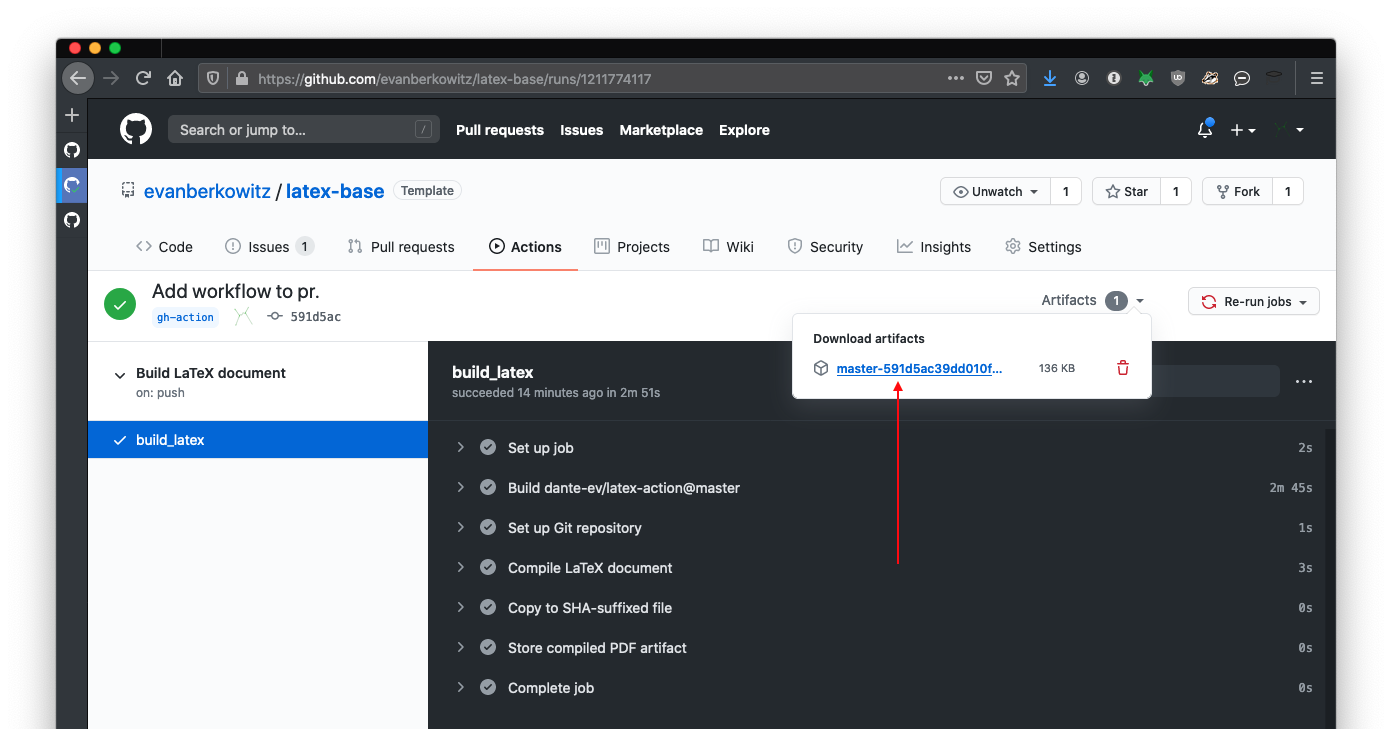
\includegraphics[width=0.75\textwidth]{figure/github-action-artifact}
\end{center}
To turn off the repository information printed on the side of the PDF, add \texttt{FINAL=1} to the \texttt{args} of the \texttt{latex-action} step of the \href{https://github.com/evanberkowitz/latex-base/blob/master/.github/workflows/main.yml}{.github/workflows/main.yml}.

On a \texttt{pull\_request} we also produce an artifact showing the diffs between the \texttt{BASE} and \texttt{HEAD}.
The action \href{https://github.com/evanberkowitz/latex-base/blob/master/.github/workflows/diff.yml}{\texttt{.github/workflows/diff.yml}} uses \texttt{git-latexdiff}~\cite{git-latexdiff} to show the differences between the two versions to be reconciled.

\section{Protected Branches}\label{sec:protected branches}

A \emph{protected branch} is a branch hosted on GitHub which users are prevented from editing freely~\cite{protected-branches}.
For example, you may want to guarantee that the revisions are always reviewed by another author before committing them.

One way to use this feature is to have a common branch from which all changes should be branched---say, the \texttt{master} branch.
To make an edit, a user branches off of \texttt{master} to create a \texttt{topic} branch.
They edit on that branch, and when they are satisfied they make a \href{https://docs.github.com/en/free-pro-team@latest/github/collaborating-with-issues-and-pull-requests/about-pull-requests}{\texttt{pull request}}.
Then, another collaborator can review those changes and approve them, or request changes.
The author of the changes can continue to make edits by pushing the same branch; on each push the GitHub Actions are run.

You can set up your repository so that \href{https://docs.github.com/en/free-pro-team@latest/github/administering-a-repository/about-required-status-checks}{passing status checks is required} or you can be more lax.
The policies are yours to determine.
When everybody is happy, the \texttt{topic} branch may be merged into the \texttt{master} branch.


\bibliography{master}

\end{document}
